% Created by tikzDevice version 0.12.6 on 2024-05-22 14:30:59
% !TEX encoding = UTF-8 Unicode
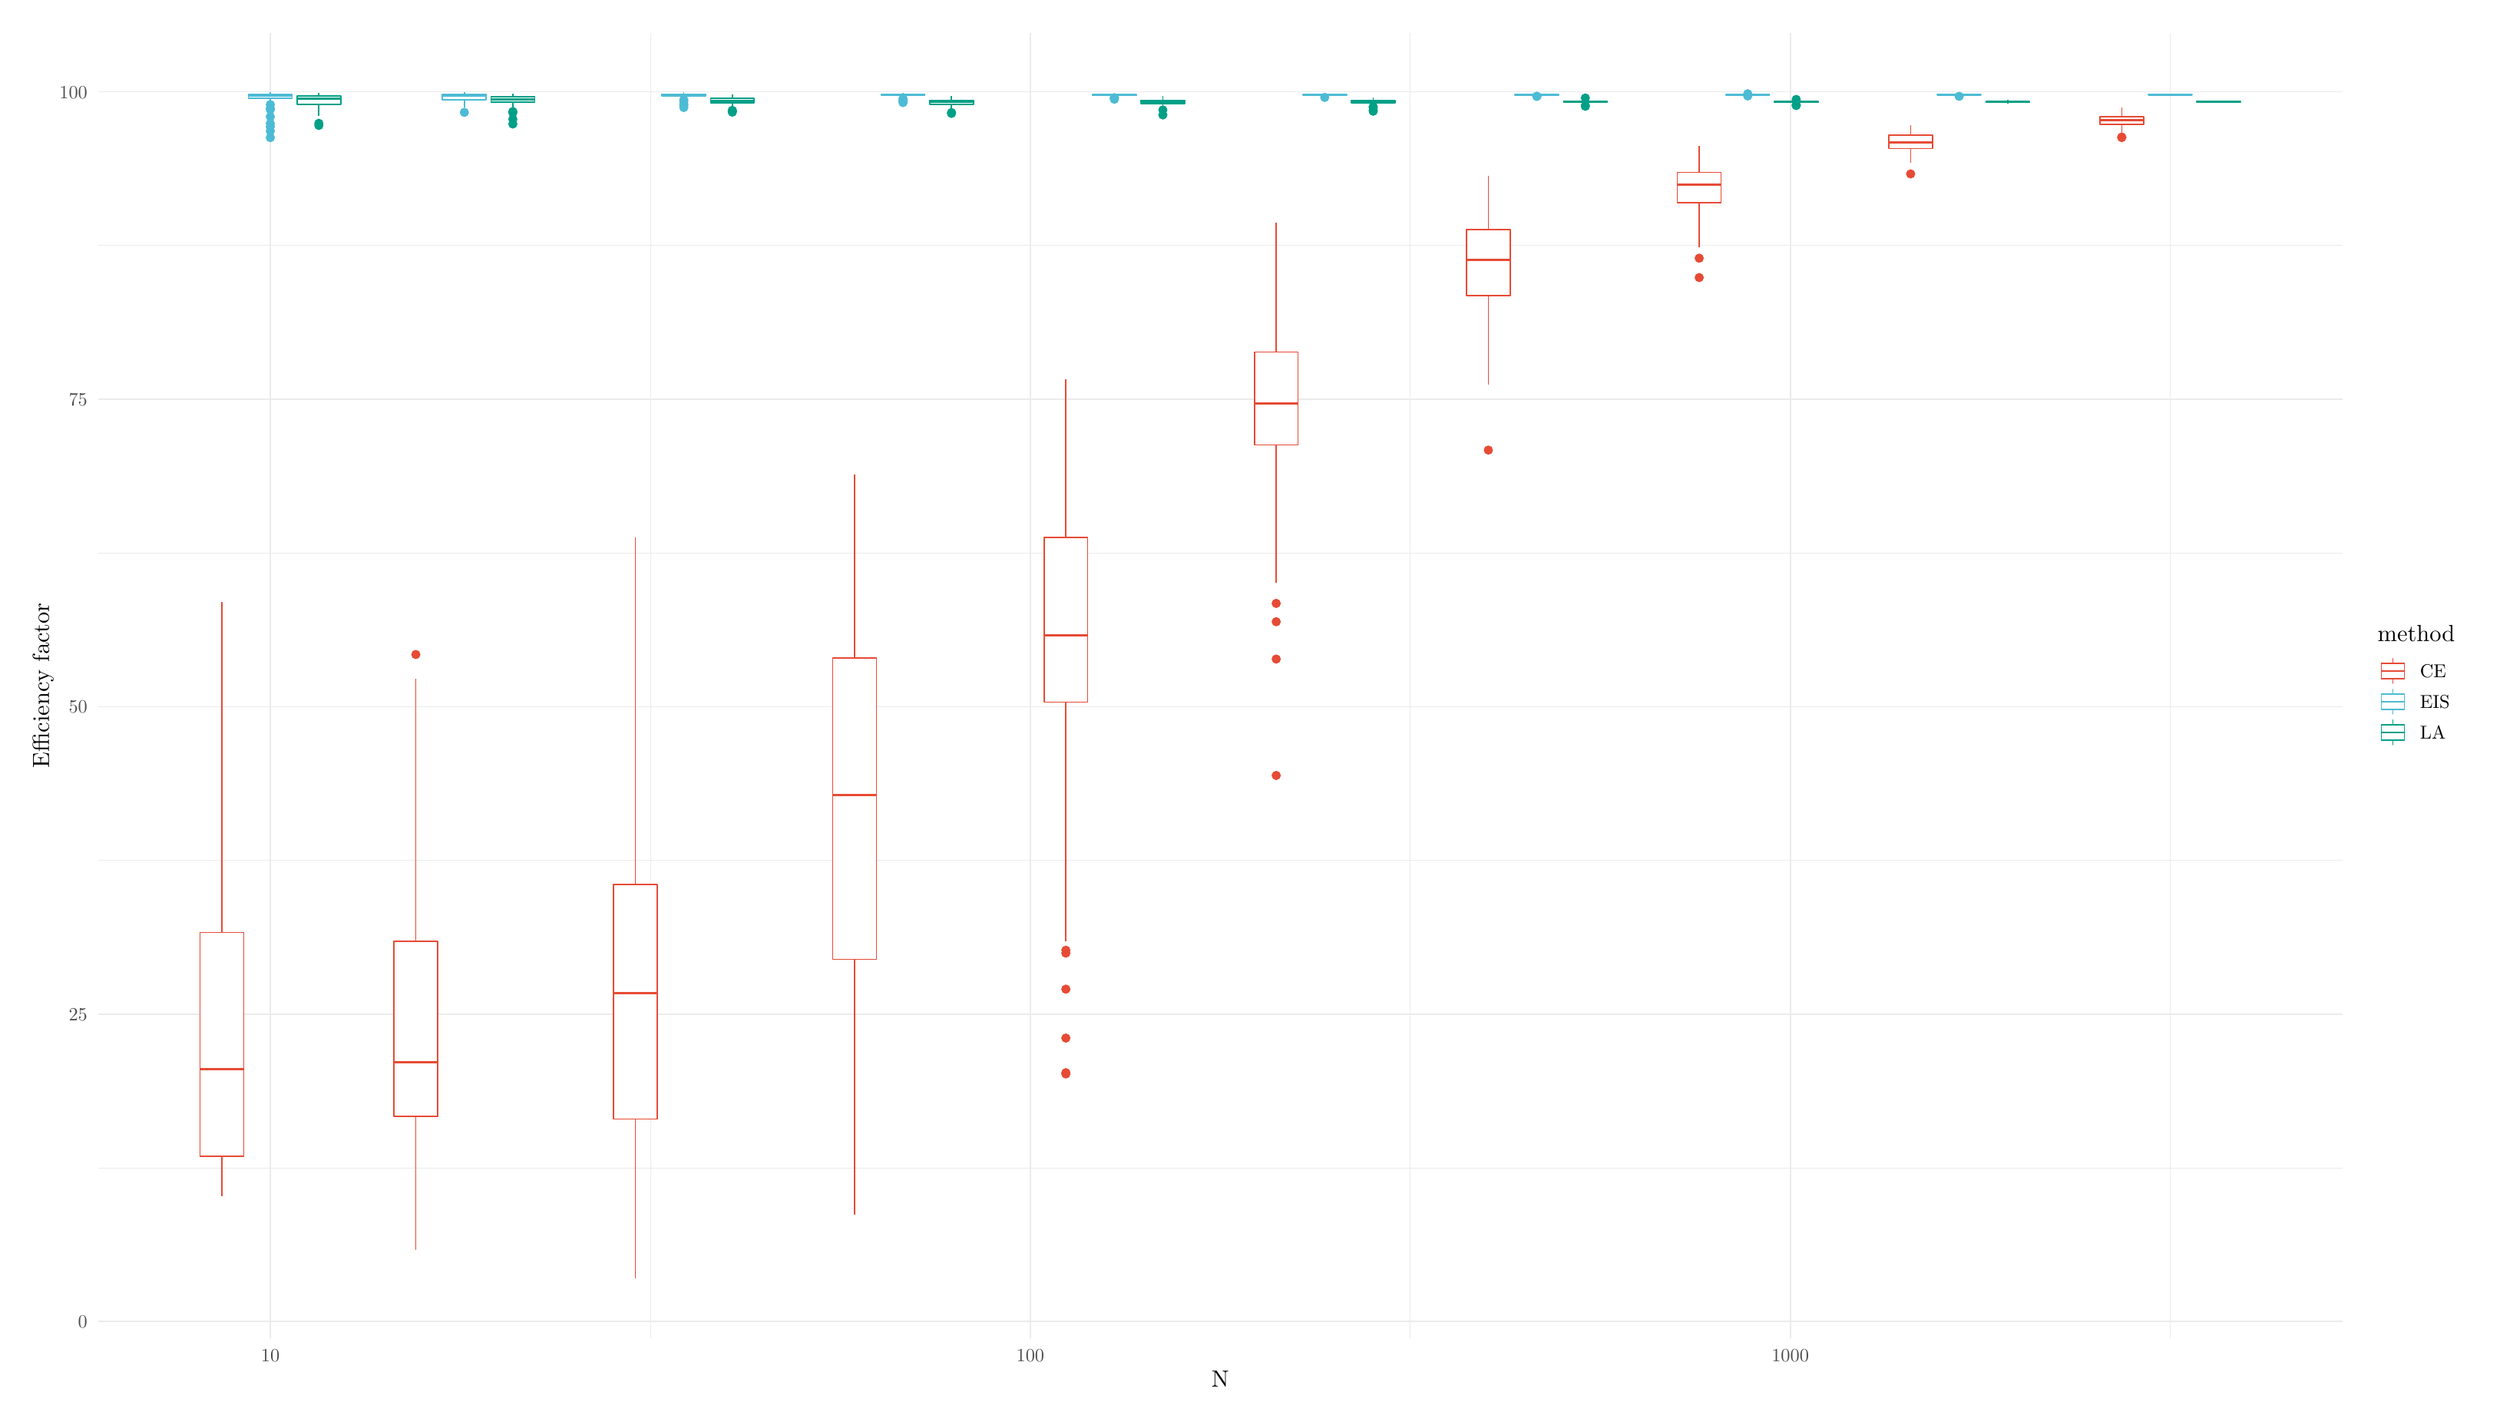
\begin{tikzpicture}[x=1pt,y=1pt]
\definecolor{fillColor}{RGB}{255,255,255}
\path[use as bounding box,fill=fillColor,fill opacity=0.00] (0,0) rectangle (1156.32,650.43);
\begin{scope}
\path[clip] ( 36.11, 30.69) rectangle (1092.47,644.93);
\definecolor{drawColor}{gray}{0.92}

\path[draw=drawColor,line width= 0.3pt,line join=round] ( 36.11,110.84) --
	(1092.47,110.84);

\path[draw=drawColor,line width= 0.3pt,line join=round] ( 36.11,255.51) --
	(1092.47,255.51);

\path[draw=drawColor,line width= 0.3pt,line join=round] ( 36.11,400.18) --
	(1092.47,400.18);

\path[draw=drawColor,line width= 0.3pt,line join=round] ( 36.11,544.84) --
	(1092.47,544.84);

\path[draw=drawColor,line width= 0.3pt,line join=round] (296.05, 30.69) --
	(296.05,644.93);

\path[draw=drawColor,line width= 0.3pt,line join=round] (653.71, 30.69) --
	(653.71,644.93);

\path[draw=drawColor,line width= 0.3pt,line join=round] (1011.37, 30.69) --
	(1011.37,644.93);

\path[draw=drawColor,line width= 0.6pt,line join=round] ( 36.11, 38.51) --
	(1092.47, 38.51);

\path[draw=drawColor,line width= 0.6pt,line join=round] ( 36.11,183.17) --
	(1092.47,183.17);

\path[draw=drawColor,line width= 0.6pt,line join=round] ( 36.11,327.84) --
	(1092.47,327.84);

\path[draw=drawColor,line width= 0.6pt,line join=round] ( 36.11,472.51) --
	(1092.47,472.51);

\path[draw=drawColor,line width= 0.6pt,line join=round] ( 36.11,617.18) --
	(1092.47,617.18);

\path[draw=drawColor,line width= 0.6pt,line join=round] (117.22, 30.69) --
	(117.22,644.93);

\path[draw=drawColor,line width= 0.6pt,line join=round] (474.88, 30.69) --
	(474.88,644.93);

\path[draw=drawColor,line width= 0.6pt,line join=round] (832.54, 30.69) --
	(832.54,644.93);
\definecolor{drawColor}{RGB}{230,75,53}

\path[draw=drawColor,line width= 0.6pt,line join=round] ( 94.40,221.61) -- ( 94.40,377.30);

\path[draw=drawColor,line width= 0.6pt,line join=round] ( 94.40,116.20) -- ( 94.40, 97.39);
\definecolor{fillColor}{RGB}{255,255,255}

\path[draw=drawColor,line width= 0.6pt,line join=round,line cap=round,fill=fillColor] ( 84.13,221.61) --
	( 84.13,116.20) --
	(104.67,116.20) --
	(104.67,221.61) --
	( 84.13,221.61) --
	cycle;

\path[draw=drawColor,line width= 1.1pt,line join=round] ( 84.13,157.37) -- (104.67,157.37);
\definecolor{fillColor}{RGB}{230,75,53}

\path[draw=drawColor,line width= 0.4pt,line join=round,line cap=round,fill=fillColor] (185.70,352.39) circle (  1.96);

\path[draw=drawColor,line width= 0.6pt,line join=round] (185.70,217.41) -- (185.70,340.90);

\path[draw=drawColor,line width= 0.6pt,line join=round] (185.70,134.98) -- (185.70, 72.05);
\definecolor{fillColor}{RGB}{255,255,255}

\path[draw=drawColor,line width= 0.6pt,line join=round,line cap=round,fill=fillColor] (175.43,217.41) --
	(175.43,134.98) --
	(195.97,134.98) --
	(195.97,217.41) --
	(175.43,217.41) --
	cycle;

\path[draw=drawColor,line width= 1.1pt,line join=round] (175.43,160.48) -- (195.97,160.48);

\path[draw=drawColor,line width= 0.6pt,line join=round] (288.99,244.06) -- (288.99,407.36);

\path[draw=drawColor,line width= 0.6pt,line join=round] (288.99,133.75) -- (288.99, 58.61);

\path[draw=drawColor,line width= 0.6pt,line join=round,line cap=round,fill=fillColor] (278.72,244.06) --
	(278.72,133.75) --
	(299.26,133.75) --
	(299.26,244.06) --
	(278.72,244.06) --
	cycle;

\path[draw=drawColor,line width= 1.1pt,line join=round] (278.72,193.04) -- (299.26,193.04);

\path[draw=drawColor,line width= 0.6pt,line join=round] (392.15,350.66) -- (392.15,436.96);

\path[draw=drawColor,line width= 0.6pt,line join=round] (392.15,208.94) -- (392.15, 88.65);

\path[draw=drawColor,line width= 0.6pt,line join=round,line cap=round,fill=fillColor] (381.88,350.66) --
	(381.88,208.94) --
	(402.42,208.94) --
	(402.42,350.66) --
	(381.88,350.66) --
	cycle;

\path[draw=drawColor,line width= 1.1pt,line join=round] (381.88,286.19) -- (402.42,286.19);
\definecolor{fillColor}{RGB}{230,75,53}

\path[draw=drawColor,line width= 0.4pt,line join=round,line cap=round,fill=fillColor] (491.61,155.58) circle (  1.96);

\path[draw=drawColor,line width= 0.4pt,line join=round,line cap=round,fill=fillColor] (491.61,211.85) circle (  1.96);

\path[draw=drawColor,line width= 0.4pt,line join=round,line cap=round,fill=fillColor] (491.61,213.20) circle (  1.96);

\path[draw=drawColor,line width= 0.4pt,line join=round,line cap=round,fill=fillColor] (491.61,194.89) circle (  1.96);

\path[draw=drawColor,line width= 0.4pt,line join=round,line cap=round,fill=fillColor] (491.61,171.86) circle (  1.96);

\path[draw=drawColor,line width= 0.4pt,line join=round,line cap=round,fill=fillColor] (491.61,154.97) circle (  1.96);

\path[draw=drawColor,line width= 0.6pt,line join=round] (491.61,407.44) -- (491.61,481.95);

\path[draw=drawColor,line width= 0.6pt,line join=round] (491.61,329.99) -- (491.61,217.56);
\definecolor{fillColor}{RGB}{255,255,255}

\path[draw=drawColor,line width= 0.6pt,line join=round,line cap=round,fill=fillColor] (481.34,407.44) --
	(481.34,329.99) --
	(501.88,329.99) --
	(501.88,407.44) --
	(481.34,407.44) --
	cycle;

\path[draw=drawColor,line width= 1.1pt,line join=round] (481.34,361.44) -- (501.88,361.44);
\definecolor{fillColor}{RGB}{230,75,53}

\path[draw=drawColor,line width= 0.4pt,line join=round,line cap=round,fill=fillColor] (590.61,376.44) circle (  1.96);

\path[draw=drawColor,line width= 0.4pt,line join=round,line cap=round,fill=fillColor] (590.61,350.24) circle (  1.96);

\path[draw=drawColor,line width= 0.4pt,line join=round,line cap=round,fill=fillColor] (590.61,367.80) circle (  1.96);

\path[draw=drawColor,line width= 0.4pt,line join=round,line cap=round,fill=fillColor] (590.61,295.46) circle (  1.96);

\path[draw=drawColor,line width= 0.6pt,line join=round] (590.61,494.77) -- (590.61,555.62);

\path[draw=drawColor,line width= 0.6pt,line join=round] (590.61,450.99) -- (590.61,386.08);
\definecolor{fillColor}{RGB}{255,255,255}

\path[draw=drawColor,line width= 0.6pt,line join=round,line cap=round,fill=fillColor] (580.34,494.77) --
	(580.34,450.99) --
	(600.88,450.99) --
	(600.88,494.77) --
	(580.34,494.77) --
	cycle;

\path[draw=drawColor,line width= 1.1pt,line join=round] (580.34,470.58) -- (600.88,470.58);
\definecolor{fillColor}{RGB}{230,75,53}

\path[draw=drawColor,line width= 0.4pt,line join=round,line cap=round,fill=fillColor] (690.44,448.59) circle (  1.96);

\path[draw=drawColor,line width= 0.6pt,line join=round] (690.44,552.27) -- (690.44,577.81);

\path[draw=drawColor,line width= 0.6pt,line join=round] (690.44,521.31) -- (690.44,479.24);
\definecolor{fillColor}{RGB}{255,255,255}

\path[draw=drawColor,line width= 0.6pt,line join=round,line cap=round,fill=fillColor] (680.17,552.27) --
	(680.17,521.31) --
	(700.71,521.31) --
	(700.71,552.27) --
	(680.17,552.27) --
	cycle;

\path[draw=drawColor,line width= 1.1pt,line join=round] (680.17,538.24) -- (700.71,538.24);
\definecolor{fillColor}{RGB}{230,75,53}

\path[draw=drawColor,line width= 0.4pt,line join=round,line cap=round,fill=fillColor] (789.68,538.91) circle (  1.96);

\path[draw=drawColor,line width= 0.4pt,line join=round,line cap=round,fill=fillColor] (789.68,529.79) circle (  1.96);

\path[draw=drawColor,line width= 0.6pt,line join=round] (789.68,579.28) -- (789.68,591.86);

\path[draw=drawColor,line width= 0.6pt,line join=round] (789.68,565.10) -- (789.68,543.98);
\definecolor{fillColor}{RGB}{255,255,255}

\path[draw=drawColor,line width= 0.6pt,line join=round,line cap=round,fill=fillColor] (779.41,579.28) --
	(779.41,565.10) --
	(799.95,565.10) --
	(799.95,579.28) --
	(779.41,579.28) --
	cycle;

\path[draw=drawColor,line width= 1.1pt,line join=round] (779.41,573.61) -- (799.95,573.61);
\definecolor{fillColor}{RGB}{230,75,53}

\path[draw=drawColor,line width= 0.4pt,line join=round,line cap=round,fill=fillColor] (889.18,578.57) circle (  1.96);

\path[draw=drawColor,line width= 0.6pt,line join=round] (889.18,596.87) -- (889.18,601.60);

\path[draw=drawColor,line width= 0.6pt,line join=round] (889.18,590.46) -- (889.18,583.72);
\definecolor{fillColor}{RGB}{255,255,255}

\path[draw=drawColor,line width= 0.6pt,line join=round,line cap=round,fill=fillColor] (878.91,596.87) --
	(878.91,590.46) --
	(899.46,590.46) --
	(899.46,596.87) --
	(878.91,596.87) --
	cycle;

\path[draw=drawColor,line width= 1.1pt,line join=round] (878.91,593.43) -- (899.46,593.43);
\definecolor{fillColor}{RGB}{230,75,53}

\path[draw=drawColor,line width= 0.4pt,line join=round,line cap=round,fill=fillColor] (988.53,595.91) circle (  1.96);

\path[draw=drawColor,line width= 0.4pt,line join=round,line cap=round,fill=fillColor] (988.53,595.67) circle (  1.96);

\path[draw=drawColor,line width= 0.6pt,line join=round] (988.53,605.61) -- (988.53,609.71);

\path[draw=drawColor,line width= 0.6pt,line join=round] (988.53,602.00) -- (988.53,597.76);
\definecolor{fillColor}{RGB}{255,255,255}

\path[draw=drawColor,line width= 0.6pt,line join=round,line cap=round,fill=fillColor] (978.26,605.61) --
	(978.26,602.00) --
	(998.80,602.00) --
	(998.80,605.61) --
	(978.26,605.61) --
	cycle;

\path[draw=drawColor,line width= 1.1pt,line join=round] (978.26,604.03) -- (998.80,604.03);
\definecolor{drawColor}{RGB}{77,187,213}
\definecolor{fillColor}{RGB}{77,187,213}

\path[draw=drawColor,line width= 0.4pt,line join=round,line cap=round,fill=fillColor] (117.22,595.66) circle (  1.96);

\path[draw=drawColor,line width= 0.4pt,line join=round,line cap=round,fill=fillColor] (117.22,611.19) circle (  1.96);

\path[draw=drawColor,line width= 0.4pt,line join=round,line cap=round,fill=fillColor] (117.22,605.53) circle (  1.96);

\path[draw=drawColor,line width= 0.4pt,line join=round,line cap=round,fill=fillColor] (117.22,598.76) circle (  1.96);

\path[draw=drawColor,line width= 0.4pt,line join=round,line cap=round,fill=fillColor] (117.22,609.48) circle (  1.96);

\path[draw=drawColor,line width= 0.4pt,line join=round,line cap=round,fill=fillColor] (117.22,602.31) circle (  1.96);

\path[draw=drawColor,line width= 0.4pt,line join=round,line cap=round,fill=fillColor] (117.22,600.79) circle (  1.96);

\path[draw=drawColor,line width= 0.4pt,line join=round,line cap=round,fill=fillColor] (117.22,608.87) circle (  1.96);

\path[draw=drawColor,line width= 0.6pt,line join=round] (117.22,616.20) -- (117.22,617.01);

\path[draw=drawColor,line width= 0.6pt,line join=round] (117.22,614.24) -- (117.22,611.55);
\definecolor{fillColor}{RGB}{255,255,255}

\path[draw=drawColor,line width= 0.6pt,line join=round,line cap=round,fill=fillColor] (106.95,616.20) --
	(106.95,614.24) --
	(127.49,614.24) --
	(127.49,616.20) --
	(106.95,616.20) --
	cycle;

\path[draw=drawColor,line width= 1.1pt,line join=round] (106.95,615.51) -- (127.49,615.51);
\definecolor{fillColor}{RGB}{77,187,213}

\path[draw=drawColor,line width= 0.4pt,line join=round,line cap=round,fill=fillColor] (208.52,607.53) circle (  1.96);

\path[draw=drawColor,line width= 0.6pt,line join=round] (208.52,616.10) -- (208.52,616.95);

\path[draw=drawColor,line width= 0.6pt,line join=round] (208.52,613.48) -- (208.52,609.97);
\definecolor{fillColor}{RGB}{255,255,255}

\path[draw=drawColor,line width= 0.6pt,line join=round,line cap=round,fill=fillColor] (198.25,616.10) --
	(198.25,613.48) --
	(218.80,613.48) --
	(218.80,616.10) --
	(198.25,616.10) --
	cycle;

\path[draw=drawColor,line width= 1.1pt,line join=round] (198.25,615.38) -- (218.80,615.38);
\definecolor{fillColor}{RGB}{77,187,213}

\path[draw=drawColor,line width= 0.4pt,line join=round,line cap=round,fill=fillColor] (311.81,611.51) circle (  1.96);

\path[draw=drawColor,line width= 0.4pt,line join=round,line cap=round,fill=fillColor] (311.81,610.98) circle (  1.96);

\path[draw=drawColor,line width= 0.4pt,line join=round,line cap=round,fill=fillColor] (311.81,609.82) circle (  1.96);

\path[draw=drawColor,line width= 0.4pt,line join=round,line cap=round,fill=fillColor] (311.81,613.50) circle (  1.96);

\path[draw=drawColor,line width= 0.4pt,line join=round,line cap=round,fill=fillColor] (311.81,612.77) circle (  1.96);

\path[draw=drawColor,line width= 0.6pt,line join=round] (311.81,616.14) -- (311.81,616.93);

\path[draw=drawColor,line width= 0.6pt,line join=round] (311.81,615.14) -- (311.81,613.71);
\definecolor{fillColor}{RGB}{255,255,255}

\path[draw=drawColor,line width= 0.6pt,line join=round,line cap=round,fill=fillColor] (301.54,616.14) --
	(301.54,615.14) --
	(322.09,615.14) --
	(322.09,616.14) --
	(301.54,616.14) --
	cycle;

\path[draw=drawColor,line width= 1.1pt,line join=round] (301.54,615.71) -- (322.09,615.71);
\definecolor{fillColor}{RGB}{77,187,213}

\path[draw=drawColor,line width= 0.4pt,line join=round,line cap=round,fill=fillColor] (414.98,612.14) circle (  1.96);

\path[draw=drawColor,line width= 0.4pt,line join=round,line cap=round,fill=fillColor] (414.98,613.96) circle (  1.96);

\path[draw=drawColor,line width= 0.4pt,line join=round,line cap=round,fill=fillColor] (414.98,613.22) circle (  1.96);

\path[draw=drawColor,line width= 0.4pt,line join=round,line cap=round,fill=fillColor] (414.98,612.65) circle (  1.96);

\path[draw=drawColor,line width= 0.6pt,line join=round] (414.98,616.17) -- (414.98,616.66);

\path[draw=drawColor,line width= 0.6pt,line join=round] (414.98,615.39) -- (414.98,614.38);
\definecolor{fillColor}{RGB}{255,255,255}

\path[draw=drawColor,line width= 0.6pt,line join=round,line cap=round,fill=fillColor] (404.71,616.17) --
	(404.71,615.39) --
	(425.25,615.39) --
	(425.25,616.17) --
	(404.71,616.17) --
	cycle;

\path[draw=drawColor,line width= 1.1pt,line join=round] (404.71,615.76) -- (425.25,615.76);
\definecolor{fillColor}{RGB}{77,187,213}

\path[draw=drawColor,line width= 0.4pt,line join=round,line cap=round,fill=fillColor] (514.43,614.25) circle (  1.96);

\path[draw=drawColor,line width= 0.4pt,line join=round,line cap=round,fill=fillColor] (514.43,614.42) circle (  1.96);

\path[draw=drawColor,line width= 0.4pt,line join=round,line cap=round,fill=fillColor] (514.43,614.32) circle (  1.96);

\path[draw=drawColor,line width= 0.4pt,line join=round,line cap=round,fill=fillColor] (514.43,613.72) circle (  1.96);

\path[draw=drawColor,line width= 0.6pt,line join=round] (514.43,616.05) -- (514.43,616.49);

\path[draw=drawColor,line width= 0.6pt,line join=round] (514.43,615.43) -- (514.43,614.51);
\definecolor{fillColor}{RGB}{255,255,255}

\path[draw=drawColor,line width= 0.6pt,line join=round,line cap=round,fill=fillColor] (504.16,616.05) --
	(504.16,615.43) --
	(524.71,615.43) --
	(524.71,616.05) --
	(504.16,616.05) --
	cycle;

\path[draw=drawColor,line width= 1.1pt,line join=round] (504.16,615.83) -- (524.71,615.83);
\definecolor{fillColor}{RGB}{77,187,213}

\path[draw=drawColor,line width= 0.4pt,line join=round,line cap=round,fill=fillColor] (613.43,614.58) circle (  1.96);

\path[draw=drawColor,line width= 0.6pt,line join=round] (613.43,616.01) -- (613.43,616.42);

\path[draw=drawColor,line width= 0.6pt,line join=round] (613.43,615.55) -- (613.43,614.93);
\definecolor{fillColor}{RGB}{255,255,255}

\path[draw=drawColor,line width= 0.6pt,line join=round,line cap=round,fill=fillColor] (603.16,616.01) --
	(603.16,615.55) --
	(623.71,615.55) --
	(623.71,616.01) --
	(603.16,616.01) --
	cycle;

\path[draw=drawColor,line width= 1.1pt,line join=round] (603.16,615.80) -- (623.71,615.80);
\definecolor{fillColor}{RGB}{77,187,213}

\path[draw=drawColor,line width= 0.4pt,line join=round,line cap=round,fill=fillColor] (713.27,615.10) circle (  1.96);

\path[draw=drawColor,line width= 0.4pt,line join=round,line cap=round,fill=fillColor] (713.27,615.07) circle (  1.96);

\path[draw=drawColor,line width= 0.6pt,line join=round] (713.27,616.04) -- (713.27,616.25);

\path[draw=drawColor,line width= 0.6pt,line join=round] (713.27,615.69) -- (713.27,615.23);
\definecolor{fillColor}{RGB}{255,255,255}

\path[draw=drawColor,line width= 0.6pt,line join=round,line cap=round,fill=fillColor] (703.00,616.04) --
	(703.00,615.69) --
	(723.54,615.69) --
	(723.54,616.04) --
	(703.00,616.04) --
	cycle;

\path[draw=drawColor,line width= 1.1pt,line join=round] (703.00,615.87) -- (723.54,615.87);
\definecolor{fillColor}{RGB}{77,187,213}

\path[draw=drawColor,line width= 0.4pt,line join=round,line cap=round,fill=fillColor] (812.51,616.31) circle (  1.96);

\path[draw=drawColor,line width= 0.4pt,line join=round,line cap=round,fill=fillColor] (812.51,615.25) circle (  1.96);

\path[draw=drawColor,line width= 0.6pt,line join=round] (812.51,615.96) -- (812.51,616.19);

\path[draw=drawColor,line width= 0.6pt,line join=round] (812.51,615.73) -- (812.51,615.40);
\definecolor{fillColor}{RGB}{255,255,255}

\path[draw=drawColor,line width= 0.6pt,line join=round,line cap=round,fill=fillColor] (802.24,615.96) --
	(802.24,615.73) --
	(822.78,615.73) --
	(822.78,615.96) --
	(802.24,615.96) --
	cycle;

\path[draw=drawColor,line width= 1.1pt,line join=round] (802.24,615.85) -- (822.78,615.85);
\definecolor{fillColor}{RGB}{77,187,213}

\path[draw=drawColor,line width= 0.4pt,line join=round,line cap=round,fill=fillColor] (912.01,615.09) circle (  1.96);

\path[draw=drawColor,line width= 0.6pt,line join=round] (912.01,615.97) -- (912.01,616.08);

\path[draw=drawColor,line width= 0.6pt,line join=round] (912.01,615.79) -- (912.01,615.59);
\definecolor{fillColor}{RGB}{255,255,255}

\path[draw=drawColor,line width= 0.6pt,line join=round,line cap=round,fill=fillColor] (901.74,615.97) --
	(901.74,615.79) --
	(922.28,615.79) --
	(922.28,615.97) --
	(901.74,615.97) --
	cycle;

\path[draw=drawColor,line width= 1.1pt,line join=round] (901.74,615.86) -- (922.28,615.86);

\path[draw=drawColor,line width= 0.6pt,line join=round] (1011.36,615.96) -- (1011.36,616.09);

\path[draw=drawColor,line width= 0.6pt,line join=round] (1011.36,615.83) -- (1011.36,615.63);

\path[draw=drawColor,line width= 0.6pt,line join=round,line cap=round,fill=fillColor] (1001.08,615.96) --
	(1001.08,615.83) --
	(1021.63,615.83) --
	(1021.63,615.96) --
	(1001.08,615.96) --
	cycle;

\path[draw=drawColor,line width= 1.1pt,line join=round] (1001.08,615.89) -- (1021.63,615.89);
\definecolor{drawColor}{RGB}{0,160,135}
\definecolor{fillColor}{RGB}{0,160,135}

\path[draw=drawColor,line width= 0.4pt,line join=round,line cap=round,fill=fillColor] (140.05,601.39) circle (  1.96);

\path[draw=drawColor,line width= 0.4pt,line join=round,line cap=round,fill=fillColor] (140.05,602.38) circle (  1.96);

\path[draw=drawColor,line width= 0.6pt,line join=round] (140.05,615.27) -- (140.05,616.59);

\path[draw=drawColor,line width= 0.6pt,line join=round] (140.05,611.38) -- (140.05,605.87);
\definecolor{fillColor}{RGB}{255,255,255}

\path[draw=drawColor,line width= 0.6pt,line join=round,line cap=round,fill=fillColor] (129.78,615.27) --
	(129.78,611.38) --
	(150.32,611.38) --
	(150.32,615.27) --
	(129.78,615.27) --
	cycle;

\path[draw=drawColor,line width= 1.1pt,line join=round] (129.78,613.90) -- (150.32,613.90);
\definecolor{fillColor}{RGB}{0,160,135}

\path[draw=drawColor,line width= 0.4pt,line join=round,line cap=round,fill=fillColor] (231.35,602.05) circle (  1.96);

\path[draw=drawColor,line width= 0.4pt,line join=round,line cap=round,fill=fillColor] (231.35,604.33) circle (  1.96);

\path[draw=drawColor,line width= 0.4pt,line join=round,line cap=round,fill=fillColor] (231.35,607.42) circle (  1.96);

\path[draw=drawColor,line width= 0.4pt,line join=round,line cap=round,fill=fillColor] (231.35,607.93) circle (  1.96);

\path[draw=drawColor,line width= 0.6pt,line join=round] (231.35,614.85) -- (231.35,616.31);

\path[draw=drawColor,line width= 0.6pt,line join=round] (231.35,612.27) -- (231.35,608.54);
\definecolor{fillColor}{RGB}{255,255,255}

\path[draw=drawColor,line width= 0.6pt,line join=round,line cap=round,fill=fillColor] (221.08,614.85) --
	(221.08,612.27) --
	(241.62,612.27) --
	(241.62,614.85) --
	(221.08,614.85) --
	cycle;

\path[draw=drawColor,line width= 1.1pt,line join=round] (221.08,613.62) -- (241.62,613.62);
\definecolor{fillColor}{RGB}{0,160,135}

\path[draw=drawColor,line width= 0.4pt,line join=round,line cap=round,fill=fillColor] (334.64,608.01) circle (  1.96);

\path[draw=drawColor,line width= 0.4pt,line join=round,line cap=round,fill=fillColor] (334.64,608.45) circle (  1.96);

\path[draw=drawColor,line width= 0.4pt,line join=round,line cap=round,fill=fillColor] (334.64,607.63) circle (  1.96);

\path[draw=drawColor,line width= 0.4pt,line join=round,line cap=round,fill=fillColor] (334.64,608.33) circle (  1.96);

\path[draw=drawColor,line width= 0.6pt,line join=round] (334.64,614.23) -- (334.64,615.99);

\path[draw=drawColor,line width= 0.6pt,line join=round] (334.64,611.92) -- (334.64,609.81);
\definecolor{fillColor}{RGB}{255,255,255}

\path[draw=drawColor,line width= 0.6pt,line join=round,line cap=round,fill=fillColor] (324.37,614.23) --
	(324.37,611.92) --
	(344.91,611.92) --
	(344.91,614.23) --
	(324.37,614.23) --
	cycle;

\path[draw=drawColor,line width= 1.1pt,line join=round] (324.37,612.93) -- (344.91,612.93);
\definecolor{fillColor}{RGB}{0,160,135}

\path[draw=drawColor,line width= 0.4pt,line join=round,line cap=round,fill=fillColor] (437.80,607.44) circle (  1.96);

\path[draw=drawColor,line width= 0.4pt,line join=round,line cap=round,fill=fillColor] (437.80,607.04) circle (  1.96);

\path[draw=drawColor,line width= 0.6pt,line join=round] (437.80,613.29) -- (437.80,615.13);

\path[draw=drawColor,line width= 0.6pt,line join=round] (437.80,611.16) -- (437.80,608.80);
\definecolor{fillColor}{RGB}{255,255,255}

\path[draw=drawColor,line width= 0.6pt,line join=round,line cap=round,fill=fillColor] (427.53,613.29) --
	(427.53,611.16) --
	(448.07,611.16) --
	(448.07,613.29) --
	(427.53,613.29) --
	cycle;

\path[draw=drawColor,line width= 1.1pt,line join=round] (427.53,612.61) -- (448.07,612.61);
\definecolor{fillColor}{RGB}{0,160,135}

\path[draw=drawColor,line width= 0.4pt,line join=round,line cap=round,fill=fillColor] (537.26,606.33) circle (  1.96);

\path[draw=drawColor,line width= 0.4pt,line join=round,line cap=round,fill=fillColor] (537.26,608.67) circle (  1.96);

\path[draw=drawColor,line width= 0.6pt,line join=round] (537.26,613.29) -- (537.26,615.11);

\path[draw=drawColor,line width= 0.6pt,line join=round] (537.26,611.67) -- (537.26,609.34);
\definecolor{fillColor}{RGB}{255,255,255}

\path[draw=drawColor,line width= 0.6pt,line join=round,line cap=round,fill=fillColor] (526.99,613.29) --
	(526.99,611.67) --
	(547.53,611.67) --
	(547.53,613.29) --
	(526.99,613.29) --
	cycle;

\path[draw=drawColor,line width= 1.1pt,line join=round] (526.99,612.59) -- (547.53,612.59);
\definecolor{fillColor}{RGB}{0,160,135}

\path[draw=drawColor,line width= 0.4pt,line join=round,line cap=round,fill=fillColor] (636.26,608.08) circle (  1.96);

\path[draw=drawColor,line width= 0.4pt,line join=round,line cap=round,fill=fillColor] (636.26,608.61) circle (  1.96);

\path[draw=drawColor,line width= 0.4pt,line join=round,line cap=round,fill=fillColor] (636.26,610.14) circle (  1.96);

\path[draw=drawColor,line width= 0.4pt,line join=round,line cap=round,fill=fillColor] (636.26,609.90) circle (  1.96);

\path[draw=drawColor,line width= 0.6pt,line join=round] (636.26,613.17) -- (636.26,614.44);

\path[draw=drawColor,line width= 0.6pt,line join=round] (636.26,611.97) -- (636.26,610.75);
\definecolor{fillColor}{RGB}{255,255,255}

\path[draw=drawColor,line width= 0.6pt,line join=round,line cap=round,fill=fillColor] (625.99,613.17) --
	(625.99,611.97) --
	(646.53,611.97) --
	(646.53,613.17) --
	(625.99,613.17) --
	cycle;

\path[draw=drawColor,line width= 1.1pt,line join=round] (625.99,612.76) -- (646.53,612.76);
\definecolor{fillColor}{RGB}{0,160,135}

\path[draw=drawColor,line width= 0.4pt,line join=round,line cap=round,fill=fillColor] (736.09,610.41) circle (  1.96);

\path[draw=drawColor,line width= 0.4pt,line join=round,line cap=round,fill=fillColor] (736.09,610.74) circle (  1.96);

\path[draw=drawColor,line width= 0.4pt,line join=round,line cap=round,fill=fillColor] (736.09,614.30) circle (  1.96);

\path[draw=drawColor,line width= 0.6pt,line join=round] (736.09,612.96) -- (736.09,613.81);

\path[draw=drawColor,line width= 0.6pt,line join=round] (736.09,612.16) -- (736.09,611.22);
\definecolor{fillColor}{RGB}{255,255,255}

\path[draw=drawColor,line width= 0.6pt,line join=round,line cap=round,fill=fillColor] (725.82,612.96) --
	(725.82,612.16) --
	(746.36,612.16) --
	(746.36,612.96) --
	(725.82,612.96) --
	cycle;

\path[draw=drawColor,line width= 1.1pt,line join=round] (725.82,612.62) -- (746.36,612.62);
\definecolor{fillColor}{RGB}{0,160,135}

\path[draw=drawColor,line width= 0.4pt,line join=round,line cap=round,fill=fillColor] (835.33,610.77) circle (  1.96);

\path[draw=drawColor,line width= 0.4pt,line join=round,line cap=round,fill=fillColor] (835.33,610.96) circle (  1.96);

\path[draw=drawColor,line width= 0.4pt,line join=round,line cap=round,fill=fillColor] (835.33,613.63) circle (  1.96);

\path[draw=drawColor,line width= 0.6pt,line join=round] (835.33,612.74) -- (835.33,613.26);

\path[draw=drawColor,line width= 0.6pt,line join=round] (835.33,612.16) -- (835.33,611.37);
\definecolor{fillColor}{RGB}{255,255,255}

\path[draw=drawColor,line width= 0.6pt,line join=round,line cap=round,fill=fillColor] (825.06,612.74) --
	(825.06,612.16) --
	(845.60,612.16) --
	(845.60,612.74) --
	(825.06,612.74) --
	cycle;

\path[draw=drawColor,line width= 1.1pt,line join=round] (825.06,612.54) -- (845.60,612.54);

\path[draw=drawColor,line width= 0.6pt,line join=round] (934.83,612.73) -- (934.83,613.34);

\path[draw=drawColor,line width= 0.6pt,line join=round] (934.83,612.23) -- (934.83,611.48);

\path[draw=drawColor,line width= 0.6pt,line join=round,line cap=round,fill=fillColor] (924.56,612.73) --
	(924.56,612.23) --
	(945.11,612.23) --
	(945.11,612.73) --
	(924.56,612.73) --
	cycle;

\path[draw=drawColor,line width= 1.1pt,line join=round] (924.56,612.50) -- (945.11,612.50);

\path[draw=drawColor,line width= 0.6pt,line join=round] (1034.18,612.67) -- (1034.18,613.14);

\path[draw=drawColor,line width= 0.6pt,line join=round] (1034.18,612.34) -- (1034.18,611.86);

\path[draw=drawColor,line width= 0.6pt,line join=round,line cap=round,fill=fillColor] (1023.91,612.67) --
	(1023.91,612.34) --
	(1044.45,612.34) --
	(1044.45,612.67) --
	(1023.91,612.67) --
	cycle;

\path[draw=drawColor,line width= 1.1pt,line join=round] (1023.91,612.50) -- (1044.45,612.50);
\end{scope}
\begin{scope}
\path[clip] (  0.00,  0.00) rectangle (1156.32,650.43);
\definecolor{drawColor}{gray}{0.30}

\node[text=drawColor,anchor=base east,inner sep=0pt, outer sep=0pt, scale=  0.88] at ( 31.16, 35.48) {0};

\node[text=drawColor,anchor=base east,inner sep=0pt, outer sep=0pt, scale=  0.88] at ( 31.16,180.14) {25};

\node[text=drawColor,anchor=base east,inner sep=0pt, outer sep=0pt, scale=  0.88] at ( 31.16,324.81) {50};

\node[text=drawColor,anchor=base east,inner sep=0pt, outer sep=0pt, scale=  0.88] at ( 31.16,469.48) {75};

\node[text=drawColor,anchor=base east,inner sep=0pt, outer sep=0pt, scale=  0.88] at ( 31.16,614.15) {100};
\end{scope}
\begin{scope}
\path[clip] (  0.00,  0.00) rectangle (1156.32,650.43);
\definecolor{drawColor}{gray}{0.30}

\node[text=drawColor,anchor=base,inner sep=0pt, outer sep=0pt, scale=  0.88] at (117.22, 19.68) {10};

\node[text=drawColor,anchor=base,inner sep=0pt, outer sep=0pt, scale=  0.88] at (474.88, 19.68) {100};

\node[text=drawColor,anchor=base,inner sep=0pt, outer sep=0pt, scale=  0.88] at (832.54, 19.68) {1000};
\end{scope}
\begin{scope}
\path[clip] (  0.00,  0.00) rectangle (1156.32,650.43);
\definecolor{drawColor}{RGB}{0,0,0}

\node[text=drawColor,anchor=base,inner sep=0pt, outer sep=0pt, scale=  1.10] at (564.29,  7.64) {N};
\end{scope}
\begin{scope}
\path[clip] (  0.00,  0.00) rectangle (1156.32,650.43);
\definecolor{drawColor}{RGB}{0,0,0}

\node[text=drawColor,rotate= 90.00,anchor=base,inner sep=0pt, outer sep=0pt, scale=  1.10] at ( 13.08,337.81) {Efficiency factor};
\end{scope}
\begin{scope}
\path[clip] (  0.00,  0.00) rectangle (1156.32,650.43);
\definecolor{drawColor}{RGB}{0,0,0}

\node[text=drawColor,anchor=base west,inner sep=0pt, outer sep=0pt, scale=  1.10] at (1108.97,358.45) {method};
\end{scope}
\begin{scope}
\path[clip] (  0.00,  0.00) rectangle (1156.32,650.43);
\definecolor{drawColor}{RGB}{230,75,53}

\path[draw=drawColor,line width= 0.6pt,line join=round,line cap=round] (1116.19,338.87) --
	(1116.19,341.04);

\path[draw=drawColor,line width= 0.6pt,line join=round,line cap=round] (1116.19,348.27) --
	(1116.19,350.44);
\definecolor{fillColor}{RGB}{255,255,255}

\path[draw=drawColor,line width= 0.6pt,line join=round,line cap=round,fill=fillColor] (1110.77,341.04) rectangle (1121.61,348.27);

\path[draw=drawColor,line width= 0.6pt,line join=round,line cap=round] (1110.77,344.65) --
	(1121.61,344.65);
\end{scope}
\begin{scope}
\path[clip] (  0.00,  0.00) rectangle (1156.32,650.43);
\definecolor{drawColor}{RGB}{77,187,213}

\path[draw=drawColor,line width= 0.6pt,line join=round,line cap=round] (1116.19,324.42) --
	(1116.19,326.59);

\path[draw=drawColor,line width= 0.6pt,line join=round,line cap=round] (1116.19,333.81) --
	(1116.19,335.98);
\definecolor{fillColor}{RGB}{255,255,255}

\path[draw=drawColor,line width= 0.6pt,line join=round,line cap=round,fill=fillColor] (1110.77,326.59) rectangle (1121.61,333.81);

\path[draw=drawColor,line width= 0.6pt,line join=round,line cap=round] (1110.77,330.20) --
	(1121.61,330.20);
\end{scope}
\begin{scope}
\path[clip] (  0.00,  0.00) rectangle (1156.32,650.43);
\definecolor{drawColor}{RGB}{0,160,135}

\path[draw=drawColor,line width= 0.6pt,line join=round,line cap=round] (1116.19,309.97) --
	(1116.19,312.13);

\path[draw=drawColor,line width= 0.6pt,line join=round,line cap=round] (1116.19,319.36) --
	(1116.19,321.53);
\definecolor{fillColor}{RGB}{255,255,255}

\path[draw=drawColor,line width= 0.6pt,line join=round,line cap=round,fill=fillColor] (1110.77,312.13) rectangle (1121.61,319.36);

\path[draw=drawColor,line width= 0.6pt,line join=round,line cap=round] (1110.77,315.75) --
	(1121.61,315.75);
\end{scope}
\begin{scope}
\path[clip] (  0.00,  0.00) rectangle (1156.32,650.43);
\definecolor{drawColor}{RGB}{0,0,0}

\node[text=drawColor,anchor=base west,inner sep=0pt, outer sep=0pt, scale=  0.88] at (1128.92,341.62) {CE};
\end{scope}
\begin{scope}
\path[clip] (  0.00,  0.00) rectangle (1156.32,650.43);
\definecolor{drawColor}{RGB}{0,0,0}

\node[text=drawColor,anchor=base west,inner sep=0pt, outer sep=0pt, scale=  0.88] at (1128.92,327.17) {EIS};
\end{scope}
\begin{scope}
\path[clip] (  0.00,  0.00) rectangle (1156.32,650.43);
\definecolor{drawColor}{RGB}{0,0,0}

\node[text=drawColor,anchor=base west,inner sep=0pt, outer sep=0pt, scale=  0.88] at (1128.92,312.72) {LA};
\end{scope}
\end{tikzpicture}
